 %\documentclass[wcp,gray]{jmlr} % test grayscale version
 %\documentclass[wcp]{jmlr}% former name JMLR W\&CP
\documentclass[pmlr,x11names,,table]{jmlr}% new name PMLR (Proceedings of Machine Learning)

 % The following packages will be automatically loaded:
 % amsmath, amssymb, natbib, graphicx, url, algorithm2e

 %\usepackage{rotating}% for sideways figures and tables
\usepackage{longtable}% for long tables

 % The booktabs package is used by this sample document
 % (it provides \toprule, \midrule and \bottomrule).
 % Remove the next line if you don't require it.
\usepackage{booktabs}
 % The siunitx package is used by this sample document
 % to align numbers in a column by their decimal point.
 % Remove the next line if you don't require it.
\usepackage[load-configurations=version-1]{siunitx} % newer version
 %\usepackage{siunitx}
 \usepackage{floatrow}



% \documentclass[11pt, oneside]{article}

%\usepackage{geometry}
%\geometry{letterpaper}

\usepackage{subcaption}
\usepackage{graphicx}
\usepackage{color}
\usepackage{xcolor}
\usepackage{amssymb}
\usepackage{hyperref,cleveref}
\usepackage{comment}

\newcommand{\templatedoc}[1]{{\color{gray}:#1}}

% add other people here 

\newcommand{\harsha}[1]{{\color{green!40!blue}[\textbf{Harsha}:#1]}}
\newcommand{\martin}[1]{{\color{blue!20!red}[\textbf{Martin}:#1]}}
\newcommand{\matthijs}[1]{{\color{blue}[\textbf{Matthijs}:#1]}}
\newcommand{\georgew}[1]{{\color{orange}[\textbf{GeorgeW}:#1]}}
\newcommand{\dmitry}[1]{{\color{blue!50!purple}[\textbf{Dmitry}:#1]}}

\iffalse 

\newcommand{\harsha}[1]{}
\newcommand{\martin}[1]{}
\newcommand{\matthijs}[1]{}

\fi


\newcommand{\eg}{\emph{e.g.}\@\xspace}
\newcommand{\etc}{\emph{etc.}\@\xspace}
\newcommand{\ie}{\emph{i.e.}\@\xspace}
\newcommand{\etal}{\emph{et al}\@\xspace}
\newcommand{\wrt}{\emph{w.r.t.}\@\xspace}


% \newtheorem{definition}{Definition}
\newcommand{\recall}[2]{${#1}$-recall$@{#2}$} 


% suggest to give it a different name compared to proposal 
\title[Billion-scale ANNS results]{Results of the NeurIPS'21 Challenge on
  Billion-Scale Approximate Nearest Neighbor Search}

 % Three or more authors with the same address:
 % \author{\Name{Author Name1} \Email{an1@sample.com}\\
 %  \Name{Author Name2} \Email{an2@sample.com}\\
 %  \Name{Author Name3} \Email{an3@sample.com}\\
 %  \Name{Author Name4} \Email{an4@sample.com}\\
 %  \Name{Author Name5} \Email{an5@sample.com}\\
 %  \Name{Author Name6} \Email{an6@sample.com}\\
 %  \Name{Author Name7} \Email{an7@sample.com}\\
 %  \Name{Author Name8} \Email{an8@sample.com}\\
 %  \Name{Author Name9} \Email{an9@sample.com}\\
 %  \Name{Author Name10} \Email{an10@sample.com}\\
 %  \Name{Author Name11} \Email{an11@sample.com}\\
 %  \Name{Author Name12} \Email{an12@sample.com}\\
 %  \Name{Author Name13} \Email{an13@sample.com}\\
 %  \Name{Author Name14} \Email{an14@sample.com}\\
 %  \addr Address}

\newcommand{\aff}[1]{\textsuperscript{#1}}

\author{%
 \Name{Harsha Vardhan Simhadri\aff{1}} \Email{harshasi@microsoft.com}\\
 \Name{George Williams\aff{2}} \Email{gwilliams@gsitechnology.com}\\
 \Name{Martin Aum\"uller\aff{3}} \Email{maau@itu.dk}\\
 \Name{Matthijs Douze\aff{4}} \Email{matthijs@fb.com}\\
 \Name{Artem Babenko\aff{5}} \Email{artem.babenko@phystech.edu}\\
 \Name{Dmitry Baranchuk\aff{5}} \Email{dbaranchuk@yandex-team.ru}\\
 \Name{Qi Chen\aff{1}} \Email{cheqi@microsoft.com}\\
 \Name{Lucas Hosseini\aff{4}} \Email{lucas.hosseini@gmail.com}\\
 \Name{Ravishankar Krishnaswamy\aff{1}} \Email{rakri@microsoft.com}\\
 \Name{Gopal Srinivasa\aff{1}} \Email{gopalsr@microsoft.com}\\
 \Name{Suhas Jayaram Subramanya\aff{6}} \Email{suhasj@cs.cmu.edu}\\
 \Name{Jingdong Wang\aff{7}} \Email{wangjingdong@baidu.com}\\
  \rm \small \\
  \aff{1} Microsoft Research 
  \aff{2} GSI Technology
  \aff{3} IT University of Copenhagen \\
  \aff{4} Meta AI Research
  \aff{5} Yandex
  \aff{6} Carnegie Mellon University
  \aff{7} Baidu
} 
 
%%\editor{Editor's name}

\iffalse 
\title{
\vspace{-40pt}
  Billion-Scale Approximate Nearest Neighbor Search Challenge}
\author{
\hspace{-20pt}  \footnotesize{Harsha Vardhan Simhadri}   \\ \hspace{-20pt} \scriptsize{Microsoft Research India} \\ \hspace{-20pt} \scriptsize{\tt harshasi@microsoft.com} \and
\hspace{-25pt}  \footnotesize{George Williams}] \\ \hspace{-25pt} \scriptsize{GSI Technology} \\ \hspace{-25pt} \scriptsize{\tt gwilliams@gsitechnology.com} \and
\hspace{-25pt}  \footnotesize{Martin Aum\"uller} \\\hspace{-30pt} \scriptsize{IT University of Copenhagen} \\ \hspace{-25pt} \scriptsize{\tt maau@itu.dk}  \and
\hspace{-20pt}  \footnotesize{Matthijs Douze} \\ \hspace{-15pt} \scriptsize{Facebook AI Research} \\ \hspace{-20pt} \scriptsize{\tt matthijs@fb.com} \and
\hspace{-25pt}  \footnotesize{Artem Babenko} \\ \hspace{-40pt} \scriptsize{Yandex} \\ \hspace{-40pt} \scriptsize{\tt artem.babenko@phystech.edu} \and
\hspace{-20pt}  \footnotesize{Dmitry Baranchuk} \\ \hspace{-20pt} \scriptsize{Yandex} \\ \hspace{-20pt} \scriptsize{\tt dbaranchuk@yandex-team.ru} \and
\hspace{-20pt}  \footnotesize{Qi Chen} \\ \hspace{-20pt} \scriptsize{Microsoft Research Asia}\\ \hspace{-20pt} \scriptsize{\tt cheqi@microsoft.com} \and
\hspace{-20pt}  \footnotesize{Lucas Hosseini} \\ \hspace{-20pt} \scriptsize{Facebook AI Research}\\ \hspace{-20pt} \scriptsize{\tt cheqi@microsoft.com} \and
\hspace{-20pt}  \footnotesize{Ravishankar Krishnaswamy} \\ \hspace{-20pt} \scriptsize{MSR India, IIT Madras} \\ \hspace{-20pt} \scriptsize{\tt rakri@microsoft.com} \and
  \footnotesize{Gopal Srinivasa} \\\scriptsize{Microsoft Research India} \\ \scriptsize{\tt gopalsr@microsoft.com} \and
  \footnotesize{Suhas Jayaram Subramanya} \\\scriptsize{Carnegie Mellon University}\\ \scriptsize{\tt suhasj@cs.cmu.edu} \and
  \footnotesize{Jingdong Wang} \\\scriptsize{Microsoft Research Asia}\\ \scriptsize{\tt jingdw@microsoft.com} 
}
%% \date{\today}
\fi

\begin{document}

\maketitle


\begin{abstract}
  Despite the broad range of algorithms for Approximate Nearest
  Neighbor Search, most empirical evaluations of algorithms have
  focused on smaller datasets, typically of 1 million
  points~\citep{Benchmark}. However, deploying recent advances in
  embedding based techniques for search, recommendation and ranking at
  scale require ANNS indices at billion, trillion or larger
  scale. Barring a few recent papers, there is limited consensus on
  which algorithms are effective at this scale vis-\`a-vis their
  hardware cost.

  This competition\footnote{\url{https://big-ann-benchmarks.com}}
  compares ANNS algorithms by hardware cost, accuracy and
  performance. We set up an open source evaluation
  framework\footnote{\url{https://github.com/harsha-simhadri/big-ann-benchmarks/}}%~\citep{framework}
  and leaderboards for both standardized and specialized hardware.
  The stadard hardware track T1 evaluates algorithms on an Azure VM
  with limited DRAM, often the bottleneck in serving billion-scale
  indices, where the embedding data can be hundreds of GigaBytes in
  size.  It uses FAISS~\citep{Faiss17} as the baseline.  The standard
  hardware track T2 additional allows inexpensive SSDs in addition to
  the limited DRAM and uses DiskANN~\citep{DiskANN19} as the baseline.
  The specialized hardware track T3 allows any hardware configuration.
  
  We compiled six diverse billion-scale datasets, four
  newly released for this competition, that span a variety of
  modalities, data types, dimensions, deep learning models, distance
  functions and sources.  The outcome of the competition was ranked
  leaderboards of algorithms in each track based on recall at a query
  throughput threshold. Additionally, for Track T3, separate
  leaderboards were also created based on recall as well as
  cost-normalized and power-normalized query throughput.
 
\end{abstract}


\begin{keywords}
Approximate nearest neighbor search, large-scale search
\end{keywords}

% !TEX root = report.tex

\section{Competition description}

Approximate Nearest Neighbor Search or ANNS is a problem of
fundamental importance to search, retrieval and recommendation.  In
this problem, we are given a dataset $P$ of points along with a
pairwise distance function, typically the $d$-dimensional Euclidean
metric or inner product with $d$ ranging from $50$ to $1000$. The
goal is to design a data structure that, given a query $q$ and a
target $k$ (or radius $r$), efficiently retrieves the $k$ nearest
neighbors of $q$ (or all points within a distance $r$ of $q$) in the
dataset $P$ according to the given distance function. In many
modern-day applications of this problem, the dataset to be indexed and
the queries are the output of a deep learning
model~\citep{deep1b-link,BERT}.  The ANNS problem is widely studied in
the algorithms, computer systems, databases, data mining, information
theory and machine learning research communities, and numerous classes
of algorithms have been developed. See, e.g.,
~\citep{CoverTree,babenko2014additive,Faiss17,Weber98,ECCV18,HNSW16,PQ11,Arya93,Indyk98,onng,scann,puffinn}
for some recent works, and also the survey
articles~\citep{samet2006foundations, LSHSurvey08, LearningToHash18,
  GraphANNSSurvey21} comparing these techniques.

However, most of the research has focused on small to medium scale
datasets of millions of vectors. For instance, the active
gold-standard benchmark site~\citep{Benchmark} that compares almost
all of the current-best ANNS algorithms \emph{uses datasets no more
  than a million points each}, and design choices in the benchmarking
system make it difficult to go beyond this scale.  Implementing most
existing state-of-art solutions for ANNS at this scale ends up being
too expensive as the indices are very RAM intensive. Alternately,
there are solutions such as SRS~\cite{Sun14} and
HD-Index~\cite{Arora18} that can serve a billion-point index in a
commodity machine, but these have high search latencies for achieving
high search accuracy.  Given the increasing relevance of search at
billion+ scale, this competition aims to rigorously benchmark the
\emph{performance of billion-scale ANNS algorithms vis-\`a-vis their
  hardware cost}.






\subsection{Tasks, application scenarios, and hardware tracks}

The main task of this challenge is to design a fast and accurate
algorithm and/or system which can build and serve a billion-vector
index with minimal hardware cost.  Specifically, this scale is a good fit
for comparing algorithmic ideas on a single machine.  Due to the
proliferation of deep-learning-based embeddings, such a system would
immediately fit into a variety of application domains, including but
not limited to web search, email search, document search, image
search; ranking and recommendation services for images, music, video,
news, etc.  To test the applicability of the submitted solutions in
these diverse use-cases, the competition run evaluations on
datasets representing these applications.


To provide a platform for the development of algorithmic and systems innovation,
the challenge introduces three different tracks: two standardized hardware tracks and 
one custom hardware track.

Most current solutions to ANNS are limited in scale as they require data
and indices to be stored in expensive main memory. We limit and
normalize the amount of DRAM available in the standardized hardware tracks
to 64GB.  Algorithms in track T1 must navigate this constraint by
efficiently compressing and indexing data much larger than the main
memory. This track thus provides a platform for algorithmic innovation 
in efficient and accurate vector quantization methods.

The second standardized hardware (T2) track incorporates 
an additional 1TB of inexpensive SSD to serve
indices. This track allows more accuracy, due to the allowance for
storing uncompressed data (the SSD is larger than all datasets in the
competition).  This track provides a platform for algorithmic
innovation for out-of-core indexing. 

In the specialized/custom hardware track T3, we encourge the use of any
existing combination of hardware or even the development of custom
hardware to solve this problem.  This aims to encourage systems
innovation to push the cost and power-normalized performance.

We summarize and provide more details on the individual tracks below.
\martin{Also specify details of index building?}


\paragraph{Track T1.}

The size of the DRAM available for serving the index is limited to
64GB. Note that in most cases, 64GB is insufficient to even host a
billion-point dataset, let alone the index, as most relevant datasets
are at least 100 dimensional and use either an {\tt int8} or a {\tt
  float32} representation of data. this means that the dataset is 100s of GB in
size.  Serving this dataset with 64GB DRAM requires compression of the
data and design the index to fit in 64GB RAM \`a la
FAISS~\cite{Faiss17}, which we use as our baseline.

\paragraph{Track T2.}

In the second set-up, the machine performing the search can rely, in addition to its 64GB RAM on a local 
solid-state drive (SSD), as is done in~\cite{DiskANN19}. 
We constrain the size of the SSD to be 1~TB and use DiskANN~\cite{DiskANN19} as the baseline.
% or 2TB?}\harsha{We have a cluster of machines with 1TB SSD. So let's go with that}


\paragraph{Track T3.}

The third set-up is the most flexible. It allows the use of more exotic 
hardware like dedicated co-processors. %% ~\matthijs{reference?}.  
This may include GPUs that aren't readily available in the major public clouds, reconfigurable hardware like FPGAs, and other custom accelerators 
available as add-on PCI boards%~\cite{amdvid,applegpu,xilinxfpga,flexfpga}
\footnote{For examples, see~\url{https://www.amd.com/en/graphics/radeon-rx-graphics},
\url{https://www.apple.com/shop/product/HM8Y2VC/A/blackmagic-egpu},
\url{https://www.xilinx.com/},
\url{https://flex-logix.com/}}.
In general, the type of hardware that can compete in T3 is not limited, but 
participants that wish to compete in T3 must first reach out to the coordinators to determine their eligibility.  Accepted T3 participants
will either 1) send us their add-on PCI boards along with installation instructions 2) if that is not possible, we will give
T3 participants the ability to run validation scripts and docker containers on their private hardware.  
%Martin: Put this discussion to metrics
%Every attempt will
%be made to ensure a fair competition among the T3 participants.  In addition to the performance benchmarks used in T1 and T2, we will declare
%winners for the following power and cost related benchmarks: \emph{(queries/second)/watt} metric and \emph{MSRP/watt}, where MSRP is the
%manufactured suggested retail price for the hardware. 
\martin{@George: Please add details how the process worked out in the end.}

\paragraph{Query types.}
We distinguish the following two query types on a dataset $S \subseteq \mathbb{R}^d$:
\begin{itemize}
  \item $k$-NN query: Given a query $q \in \mathbb{R}^d$ and an integer $k \geq 1$, return the $k$-nearest neighbors to the query point in $S$.  
  \item Range search: Given a query $q \in \mathbb{R}^d$ and a distance threshold $R$, return all points in $S$ that are at distance at most $R$ from $q$.
\end{itemize}

\subsection{Data}
The datasets in Table~\ref{table:datasets} were made available for download for the competition along with ground truth data.
We summarize these datasets in the following.

\begin{table}
  \begin{tabular}{r c c c c c}
    Dataset & Type & d & Dist. & Query Type & Reference \\\hline
    \textsf{BIGANN} &	uint8	& 128	& L2	& k-NN & \cite{SIFT1B} \\
    \textsf{Facebook SimSearchNet++} & uint8 & 256 & L2 & Range & [this paper]\\
    \textsf{Microsoft Turing-ANNS} & float32 & 100 & L2 & k-NN & [this paper] \\
    \textsf{Microsoft SPACEV} & int8 & 100 & L2 & k-NN & [this paper] \\
    \textsf{Yandex DEEP} & float32 & 96 & L2 & k-NN & \cite{deep1b-link} \\
    \textsf{Yandex Text-to-Image} & float32 & 200 & IP & k-NN & [this paper]
  \end{tabular}
  \caption{Summary of datasets.}
  \label{table:datasets}
\end{table}


% \matthijs{Maybe not useful to give the exact list of datasets for the proposal}
% \martin{Agreed, but we should stress the impact of making these dataset available}
% \harsha{Instructions ask us to comment on when data will be released and the terms. So it might be necessary to list them.}

\begin{itemize}
  \item \textsf{Microsoft Turing-ANNS} is a new dataset being released by the
    Microsoft Turing team for this competition. It consists of web
    search queries encoded by the universal language AGI/Spacev5
    model. This model is trained to capture generic intent
    representation~\cite{AGIv4} and uses the Turing-NLG
    architecture~\cite{Turing-NLG}. The query set also consists of web
    search queries, and the goal is to match them to the closest
    queries seen by the search engine in the past.
  \item \textsf{Microsoft SPACEV1B} is a new dataset being released by
    Microsoft Bing for this competition. It consists of more than one
    billion document vectors and 29K+ query vectors encoded by
    Microsoft SpaceV Superior model \martin{reference?}. This model is trained to capture
    generic intent representation for both documents and queries. The
    goal is to match the query vector to the closest document vectors
    in order to achieve top relevant documents for each query.
  \item \textsf{Facebook SimSearchNet++} is a new dataset being released by
    Facebook \martin{Meta?} for this competition. It is a dataset of image descriptors 
    used for copyright enforcement, content moderation, etc.
    Vectors should be compared with cosine distance. \martin{@Matthijs: We did l2, right?}
  \item \textsf{Yandex Text-to-Image} from Yandex is a new cross-modal dataset,
    where database and query vectors can potentially have different
    distributions in a shared representation space. The database
    consists of image embeddings produced by the Se-ResNext-101 model
    \cite{hu2018squeeze} and queries are textual embeddings produced
    by a variant of the DSSM model \cite{huang2013learning}. The
    mapping to the shared representation space is learned via
    minimizing a variant of the triplet loss using click-through data. The similarity measure for this dataset is inner product.
  \item \textsf{BIGANN} contains SIFT descriptors applied
    to 1 billion images. This is available at
    \url{http://corpus-texmex.irisa.fr/} is already used as a
    benchmark by existing algorithms. 
  \item \textsf{DEEP1B} consists of the outputs of a DNN for a
    billion images on the web, introduced in~\cite{deep1b-link} and made
    available
    \href{https://github.com/arbabenko/GNOIMI/blob/master/downloadDeep1B.py}{here}. This
    dataset is already used for benchmarking in the community.
\end{itemize}

The datasets are provided from websites managed by the data creators. 
The webpage \url{https://big-ann-benchmarks.com/} collects these and summarizes their properties.
File formats were made as uniform as possible, taking into account the fact that some datasets are 
in \texttt{float32} and others are in \texttt{uint8}.
For each dataset, we provide: 
\begin{itemize} 
  \item a set of 1 billion database vectors to index; 
	\item a set of query vectors for validation (at least 10\,000 of them); 
	\item a set of query vectors held out for the final evaluation (the same size);
	\item ground truth consisting of the 100 nearest neighbors for each query in the validation set, including results at the reduced scales of 10M and 100M vectors.
\end{itemize}
The experimental framework manages working with (variants of) these datasets automatically.

% \matthijs{For deep1B and Sift1B the challenge will be to get additional queries. Perhaps they could be sampled from the training set, that is not used otherwise in the challenge}

% \martin{We could also make noisy versions of some data points, or we make it explicit that the query points are part of the dataset. (Meaning that the nearest neighbor should always be ignored.)}
%% If the competition uses an evaluation based on the analysis of data,
%% please provide detailed information about the available data and
%% their annotations, as well as permissions or licenses to use such data.

%% If new data are collected or generated, provide details on the
%% procedure, including permissions to collect such data obtained by an
%% ethics committee, if human subjects are involved. In this case, it
%% must be clear in the document that the data will be ready prior to the
%% official launch of the competition.

%% Please justify that: (1) you have access to large
%% enough datasets to make the competition interesting and draw
%% conclusive
%%  results; (2) the data will be made freely available;(3) the ground truth has been kept confidential.


\subsection{Metrics}
\label{metrics}


The leaderboards compared the algorithms by their Pareto-optimal
curve of the recall vs throughput that they offer (using various
configuration parameters), akin to the measurements in~\cite{Benchmark}. 


% redundant with previous section
\iffalse 
The evaluation for tracks T1 and T2 will be run by the organizers on
normalized hardware.  T1: machine with 64GB RAM (memory shared by
index with OS and standard libraries); T2: same machine with an
additional 1 TB of SSD.  For T3, since the hardware is non standard,
the participants are expected run the evaluation themselves using the
evaluation scripts provided by the organizers.  Some T3 participants
may wish to send us their custom accelerator hardware for the
evaluation phase.  We will accommodate those requests on a case-by-case
basis.
\fi 

% \matthijs{For the parts below, I am not sure we need to go into that much detail for the NeurIPS proposal. Maybe move to a new doc about the contest rules for participants that we have to provide as well.}
% \martin{I agree.}



%% \noindent{\bf Recall.}
%% Depending on the use case, the requirement
%% of the ANNS system might be to retrieve candidates which are in the
%% vicinity of the true nearest neighbors, or we might require a stricter
%% guarantee on retrieving most of the desired $k$ candidates. The
%% in-memory setting that requires lossy data compression can only
%% support the former.  Hence for the leaderboards, we use different ways
%% of measuring recall: for the first category, we will measure
%% \recall{1}{k} for $k=1, 10,100$, and for the second category we will
%% measure a stronger notion of \recall{k}{k} for $k=1,10,100$. \matthijs{Not sure we need to distinguish them, I'm fine with recall k@k for both}




\noindent{\bf Throughput.} The overall query
throughput using all the threads available on the standardized machine.
All queries are provided at once, and we measure the wall clock time
between the ingestion of the vectors and when all the results are
output. The resulting measure is the number of queries per second (QPS).


%% \matthijs{There was some discussion about this. This is a scenario that is most comfortable for the API developers, because if we measure per-query latency, the parallelization becomes more tricky as we can't parallelize on queries anymore}

%%  \martin{I would probably say that they can provide a single set of parameters for index building, and a collection of 10 or so different parameters for how to answers queries using the index.}

The participants can provide one configuration for index building and
up to around 10 (final number will be decided based on compute
availability) different sets of search parameters per dataset that
will be evaluated. 
%\matthijs{Did we end up doing this?} 
%Martin: Yes!
Each set of search parameters is intended to
strike a different tradeoff in terms of accuracy vs. search time.  At
evaluation time, the sets of search parameters will be evaluated in
turn. The limited amount of hardware memory will disallow caching
of data in out-of-core track T2.


%% Between each set, the disk caches and RAM will be flushed by
%% \matthijs{Maybe reading a lot of unrelated data} \martin{I think this
%%   is only relevant on T2, and I would favor a hardware solution.}

\noindent{\bf Build time.} 
A hard time limit of 4 days per dataset for the time allowed to build an index on a standardized setup was enforced during the competition.
\matthijs{did we measure build time for the indexes or did the participants provide prebuilt indexes?}
\martin{I changed this to only mention the time limit that we eventually enforced.}

\paragraph{Search accuracy.}

Two notions of search accuracy, defined as follows,
depending on the dataset. For scenarios require $k$-NN search using
the first notion of recall, we will measure 10-recall@10, \ie 
the number of correct 10-nearest neighbors found in the $k=10$ first results.

\iffalse 

\begin{definition}[{\bf \recall{k}{k'}}]
  \label{def:recall}
  For a query vector $q$ over dataset $P$, suppose that (a) $G
  \subseteq P$ is the set of actual $k$ nearest neighbors in $P$, and
  (b) $X \subseteq P$ is the output of a $k'$-ANNS query to an index
  for $k' \geq k$ nearest neighbors. Then the \recall{k}{k'} for the
  index for query $q$ is $\frac{|X \cap G|}{k}$. Recall for a set of
  queries refers to the average recall over all queries.
\end{definition}

\fi

% \paragraph{Range search accuracy.}

A range search returns a list of database items whose length is not fixed in advance (unlike k-NN search).
We compute the ground truth range search results. 
The range search accuracy measure is the precision and recall of the algorithm's results w.r.t. the ground truth results.
We will use the average precision over recall values when clipping the result list with different values of the threshold.


\iffalse 

\begin{definition}[{\bf Range search average precision at $\epsilon$}]
  \label{def:rangeaccuracy}
  For a query vector $q$ over dataset $P$, suppose that (a) $G
  \subseteq P$ is the set of actual nearest neighbors within range $\epsilon$ 
  of the query in in $P$, and
  (b) $X \subseteq P$ is the output of a ANNS range query to an index
  for range $\epsilon'$. 
  Then the precision in $p=\frac{|X \cap G|}{|X|}$ and recall is $r=\frac{|X \cap G|}{|G|}$. 
  The accuracy measure that we use is the average precision while sweeping over $\epsilon'$ values.
\end{definition}

\fi

% \textcolor{blue}{Qi: Shall we add the resource usage into consideration? e.g. memory and disk usage. These capacity cost metrics are also very important when deploying the ANN related applications into real production environment. Maybe we should take the \#vectors/GB that the index can support into consideration?}

% \matthijs{The setting is that the type of machine imposes the resource constraint, and given that constraint we measure the speed-accuracy tradeoff. }


\paragraph{Synthetic performance measure.}

% \matthijs{Outdated: eventually we chose to use the recall at a given QPS target}

Participants will obtain several tradeoffs in the QPS-accuracy space,
where accuracy is either the 10-recall@10 (for k-NN search) or the
average precision (for range search).  
The challenge page will report
these tradeoff plots, similar to the {\tt ann-benchmarks.com}
page~\cite{Benchmark} or the Faiss benchmarks\footnote{\url{https://github.com/facebookresearch/faiss/wiki/Indexing-1G-vectors}},
for each evaluated dataset.

However, for the leaderboard we need a single scalar metric to rank the participants. 
For this we will use a synthetic accuracy metric. 
For each track, we fix a given QPS target, and read from the Pareto-optimal curve what is the maximum accuracy we can get with at least that QPS. 
%
We then average these accuracy measurements over the six datasets. 
The QPS targets are calibrated on the baseline methods described in the next section. 
For Track 1: QPS=10,000, Track 2: QPS=1,500. Track 3: QPS=\matthijs{Did we have a QPS here?}.


\iffalse 

\begin{definition}[{\bf synthetic QPS metric.}]
  \label{def:syntheticmetric}
  Given a set of $n$ QPS-accuracy operating points $\Omega = \{(q_1, a_1), ..., (q_n, a_n), (q_\mathrm{exact}, 1)\}$, 
  and a minimal accuracy threshold $A$,   the synthetic QPS measure is 
  \[
Q =  \max \{ q, \forall (q, a)\in \Omega \ \ \mathrm{st.}\ \  a\ge A \}
  \]
  where $q_\mathrm{exact}$ is the QPS of an exhaustive search on the reference machine.
\end{definition}


The rationale for including the exact-search metric is to be able to score algorithms that do not reach the required accuracy level even with their most expensive settings.
Threshold $A$ will be calibrated based on the measured accuracy of our baseline methods. 
It will be adjusted separately for the tracks T1, T2, T3, and possibly per dataset as well. 
We expect $A$ to be lower for T1 than for T2 because T1 requires a stronger compression, and thus the maximal accuracy cannot be as high as for T2.


The score over all datasets will be the geometric mean of the synthetic QPS measures of all databases:
\begin{definition}[{\bf averaged QPS metric.}]
  \label{def:averagedmetric}
  Given a set of runs of a participant that obtained synthetic QPS metrics $\{Q_1,...,Q_n\}$ on the $n$ datasets, the average metric is 
  \[
  Q_\mathrm{avg} = \left( 
\prod_{i=1..n} Q_i
  \right)^{1/n} 
  \]
\end{definition}
% 
The reason for using a geometric mean is that the QPS scale is logarithmic rather than linear~\cite{Benchmark,FaissBenchmarks}.

\fi 

\subsection{Baselines, code, and material provided}

We will use the following two baseline algorithms for the two
leaderboards.  They are both open-sourced with MIT license and well
tested in production: FAISS for in-memory indices (T1) and DiskANN for out-of-core indices (T2). 
The developers of the two libraries will propose reasonable parameterizations for both.
\iffalse 
\begin{itemize}
  \item FAISS for in-memory indices (T1). 
    \url{https://github.com/facebookresearch/faiss}
  \item DiskANN for out-of-core indices (T2).
    \url{https://github.com/microsoft/DiskANN}
\end{itemize}
\fi

% redundant
\iffalse 
In addition to the data and corresponding ground-truth listed earlier,
we will provide a 1\% and 10\% sample of the dataset (10M and
100M points respectively) for participants to develop, debug and
optimize their code with shorter turn-around times.
\fi

We also provide Azure compute credit to participants with
suggestions on virtual machine SKUs that approximate the bare-metal
hardware that will be used in the final evaluation.  Participants who
want to work with alternative hardware configuration (for example a
GPU) are allowed to use a SKU of their choice for (T3).


Extending the techniques used in the evaluation framework~\cite{Benchmark}, 
we provide a standard benchmarking framework in which participants can 
run their code.
The framework takes care of downloading and preparing the datasets,
running the experiments for a given implementation, 
and evaluating the result of the experiment in terms of the metrics mentioned above.
We showcase the framework using the two baselines from above.


\begin{comment}
  
\subsubsection{New Scenarios and Requirements}  \label{sec:scenarios}

Traditional search techniques rely on structured data, literal matches
and database queries.  However, numerous advances in machine learning
have led to the popularity of embedding-based techniques for many
tasks in natural language processing, computer vision and speech
domains.  Here ANNS is typically used to search a large pool of
data points for the most relevant candidates for a query. The pool that
is queried is often extremely large, spanning \emph{billions or even
  trillions of vectors}. A few such examples include:
\begin{itemize}
  \item Document Ranking: Retrieve the most appropriate document for a
    user query from a large corpus~\cite{trec19dl}.
  \item Question Answering: Highlight the sentence or paragraph from a
    large knowledge store (e.g. Wikipedia) that best answers a
    question.
  \item Entity Linking: Match user query to a database of known entities~\cite{bennett2007netflix}.
  \item Ads retrieval: Match user query to a database of Ad keywords~\cite{twinbert20}.
  \item Image match: Find the best match to an image from a pool of
    known images~\cite{douze2016polysemous,FBAI2020covidmisinfo}.
  \item Text to Image search: Find the images that best match a given query.
  \item Map match: Find the best match to a picture from satellite data.
  \item Extreme Classification: Find appropriate labels from amongst a
    billion for a data point (labels here can be text categories,
    relevant pages, users,
    etc.)~\cite{jain2019slice,nigam2019semantic, DeepXML21, GalaXC21}.
  \item Link prediction using graph embeddings. 
  \item Contrastive Sampling: find hard negatives for training models
    using sparse data~\cite{conneau2017word, ance20}.
  \item Molecule Similarity Search. Find structurally similar
    molecules to a virtual query molecule in computational drug
    discovery~\cite{pmlr-v119-ryali20a,Samanta2020.06.26.172908,C7SC02664A}.
\end{itemize}




 

%% At a high level, the quality of the system is measured by the search
%% latency achievable for a desired recall target, and the cost of
%% running the system is the total hardware cost of the components used
%% by the system.

\subsection{Impact}

\matthijs{reduce or remove this section?}

Our ultimate goal from the Big-ANNS challenge is that we will uncover
\emph{newer and more efficient ANNS systems} for billion-scale ANNS, a
very important real-world problem cutting across application
domains. Moreover, by not restricting the machine configuration to a
fixed type, and by allowing different kinds of hardware configurations in \emph{separate tracks of the competition}
(subject to the cost considerations), we hope that there might be new
ideas proposed which can leverage novel configurations to provide
cost-effective and high-quality indices. 
Overall, we believe that the goal of permanently hosting and maintaining a leaderboard of the most cost-efficient billion-scale ANNS solutions  will not only advance the state-of-the-art for large-scale ANNS, it will also
\emph{democratize the applicability of this problem}, given that it is
prohibitively expensive for many end-users to deploy existing
fast-and-accurate ANNS to large-scale indices they might have.
Another lasting impact is that we plan for the Big-ANNS
competition to be a \emph{permanent one-stop repository} of
billion-scale datasets which we will carefully compile from the various
real-world scenarios listed in~\Cref{sec:scenarios}. 
Lastly, we believe that our Big-ANNS competition will serve as a standard evaluation framework for 
ANNS algorithms on that scale, which will outlive the competition.
In short, we can categorize the
impact of the Big-ANNS challenge as follows:

\begin{itemize}
	\item A comparative understanding of algorithmic ideas and their
	application at scale.
	\item Development of new techniques for the problem and demonstration
	of their value.
	\item A compilation of datasets to enable future development of algorithms.
  \item Introduction of a standard benchmarking approach.
\end{itemize}

We also believe that by unifying many of the interested parties in
this problem (ranging from theory to possible applications), we will
\emph{foster more cross-collaboration} and collectively advance the
field at a more rapid pace.  

Going forward, another possible extension
of the challenge, which could be considered beyond this year's
competition, is the case of serving ANNS queries over \emph{dynamic
  datasets that change over time}. Maintaining dynamic indices in
general is not as well understood as the indices for static datasets,
again with the usual tradeoff between quality and the cost to maintain
such a dynamic system.


  
\subsubsection{Relevance to NeurIPS community}

ANNS is a topic that is both actively developed and used in many publications each year.
Recent research directions include:
\begin{itemize}
\item
     hash-based methods like \cite{kulis2009learning}
\item
	 graph-based methods like \cite{WangL12, WangWZTGL12}, HNSW~\cite{HNSW16}, NSG~\cite{NSG17}, SPTAG~\cite{ChenW18}, ONNG~\cite{onng}
\item 
	hardware PQ implementations~\cite{Andre_2019}
\item
	better quantization methods~\cite{scann}
\item 
	learned distance metrics~\cite{sablayrolles2019spreading,baranchuk2019learning} and learned indices~\cite{DBLP:conf/iclr/DongIRW20}
\item 
 	external-memory-based methods like Flash/RAM (DiskANN)~\cite{DiskANN19}, far-memory/RAM~\cite{hm-ann20} and specialized SRAM memory such as that you might find in 
FPGA and custom in-memory processors~\cite{10.1007/978-3-030-27562-4_27,ZhangJialiang}.
\item
	GPU-based methods like~\cite{Faiss17,DBLP:conf/sigmod/WangSWR18,groh2019ggnn}
\item using ANNS methods to speed-up ML training~\cite{DBLP:conf/mlsys/ChenMFGTS20, chen2021mongoose}

\item search with non-metric distance~\cite{Shrivastava014} (Best paper award NeurIPS 2014)
\end{itemize}

Many of these
works~\cite{kulis2009learning,Shrivastava014,DiskANN19,hm-ann20} are
published in NeurIPS.  In addition, many practitioners in this
community, especially from industry, use these algorithms regularly.



\subsection{Novelty}
At a high-level, the Big-ANNS competition is closely related to the
benchmarking efforts on the website \url{ann-benchmarks.com}~\cite{Benchmark} in that it allows comparisons of
recall vs latency properties of algorithms without a memory
budget. However, the proposed competition is novel in several
regards. It is the first evaluation on datasets spanning
\emph{billions of vectors} from real-world scenarios, with existing
benchmarks topping at around million vectors. Secondly, and equally
importantly, it is the first comprehensive evaluation of the trade-off
between quality of the ANNS system and its \emph{hardware cost}. The
existing benchmark site allows any algorithm which can build and serve
the index in a certain fixed SKU\footnote{Stock Keeping Units. Used here in reference to cloud virtual machines of a certain configuration}, and does not differentiate between
algorithms which use the entire resource and those which use a tenth
of the allotted SKU.

Our competition also be the first effort to bring together most
leading efforts for this problem from academia and industry which we
hope will advance state-of-the-art significantly. Another novelty is
that we also \emph{intend to actively welcome solutions} and proposals
from more \emph{financially-constrained participants}, by providing
compute credits for the required SKUs, provided the solutions meet
certain qualifying criteria on medium-scale datasets. Lastly, as
mentioned before, another novelty of this effort is to collect
large-scale real-world datasets from various industrial labs where
they play a crucial role in various application domains.

\end{comment}


%% Specify what are (will be) the baselines for the competition. Provide preliminary results, if available.

%% Indicate
%% whether there will be available code for the participants to get started with (``starting kit''). For certain competitions, material provided may include a hardware platform.

%% \subsection{Tutorial and documentation}

%% We think the problem is self-explanatory. We will provide links to
%% papers and code to the algorithms that have already been developed for this
%% problem. Furthermore, the evaluation framework will provide plenty 
%% of examples to allow teams to start working on their competition entries.


%% Provide a reference to a white paper you wrote describing the
%% problem and/or explain what tutorial material you will provide.


% !TEX root = proposal.tex



\section{Organizational aspects}
\subsection{Protocol}

%% Explain the procedure of the competition: what the participants will
%% have to do, what will be submitted (results or code), and the
%% evaluation procedure.  Will there be several phases? Will you use a
%% competition platform with on-line submissions and a leader board?
%% Indicate means of preventing cheating.  Provide your plan to organize
%% beta tests of your protocol and/or platform.



The competition consists of the following phases:
\begin{itemize}
\item Participants enter the competition by submitting an expression
  of interest along with the team information. Teams requesting
  compute credits will be additionally required to submit a short
  overview of the ideas to be explored, their novelty, and share any
  experimental data on the smaller slices (10M, 100M points) of the
  datasets to back the merits of the proposal. We will use this
  proposal to screen for serious attempts and limit fragmenting
  limited compute credits.
\item Participants start iterating on ideas, and submit their code in private
  (e.g. by providing read access to a private repo), with support for
  a standard interface that the evaluation platform can invoke, if
  they want their entry up on the leaderboard.
\item At the end of the competition period, participants are expected
  to release their code for transparency and open discussion, and
  submit a short report on their algorithm and the results obtained.
\item In the final phase leading up to NeurIPS'21, the organizers will
  run the code provided on a standardized set of machines, and post
  the results to the final leaderboard.
\end{itemize}

Before the start of competitions, we will release the datasets, set up
the baseline algorithms along with wrappers that automate the process
of downloading the dataset to a local drive, building an index, and
then searching the query set. Organizers will beta test this before
release and we expect that participants can copy and adapt the wrapper
code.  Based on data generated by automated scripts, we will populate
the leaderboard.


\subsection{Rules}


%% \martin{\url{https://arxiv.org/pdf/2012.07976.pdf} is a nice reference.}

\paragraph{Draft of Rules.} 

These rules apply mainly to tracks T1 and T2. 
Due to the hardware constraints of T3, there is a specific set of rules for that track.

\begin{enumerate}
  \item Participants are expected to form teams.  There are no limits
    on the number of participants in each team. % \matthijs{is it useful to distinguish individual participants from teams?} 
\item Each participant can only be in one team.
\item Each team might apply to access computing units if they lack the
  infrastructure or budget for development. Organizers will decide
  distribute compute credit to support a diverse set of participants
  from across the world. We will also offer suggestions on setting up
  Azure VMs to maximize experimentation possibilities to new teams
  starting up.
\item Each team needs to publish their submission code to a public
  repository to be included in the final evaluation.  Participants are
  also required to write a wrapper for the evaluation platform and
  contribute a set of parameters.
  \item The submitted code will be in a Docker container, that provides a
    command line utility with predefined flags to run the indexing and
    search.
  \item All teams that want to be evaluated in the final phase must
    submit their implementation with parameter choices that build an
    index on the BIGANN dataset points within a time limit of 3
    days on a specified SKU of Azure VM. Otherwise, the entry will be judged as TLE (timelimit
    exceeded). The team is required to make sure that the index can
    be build in the allotted time.
\item A maximum of 10 parameter choices can be provided for evaluation
  of search performance. The Pareto-optimal parameter choices and the
  results obtained with them will be published.
  \item The evaluation in the final phase will be carried out on
    bare-metal machines in control of the organizers. Hardware details
    have to be fixed, but we will use mid-range workstations with
    commodity hardware so that the results are indicative of the
    algorithm's performance without the need for cutting edge or
    expensive hardware.  Organizers will suggest similar cloud units
    for testing.
  %% \item In the final phase, each team is allowed to specify a single
  %%   set of parameters used for building the index, i.e., build a
  %%   single index per dataset, and provide at most 10 query
  %%   parameters.   \item A team submitting code that (explicitly) tries to cache the results of queries will be disqualified.
  \item 
    In the leaderboard, participants will be ranked based on the average QPS measure $Q_\mathrm{avg}$ (Definition~\ref{def:averagedmetric}).
      \item Each team needs to submit a report that describes details of
    the solution to be eligible for winning in Phase 3. This will be
    released to the public to share the learning from the competition.

%%  \item In the final phase, each team is allowed to specify a single set of parameters used for building the index, i.e., build a single index per dataset, and provide at most 10 query parameters. The team is required to make sure that the index can be built in the allotted time. 
  \item A team submitting code that (explicitly) tries to cache the results of queries will be disqualified.
  \item Co-organizers of this competition are allowed to participate, but are not included in the final ranking.
  \item No prize money will be awarded. 
\end{enumerate}

%% \martin{If we add prize money, there is usually a large chunk of legal terms to be added.} 


\paragraph{Discussion of Rules.}  
Our primary goal is to motivate researchers and practitioners in
industry to try out the ideas for nearest-neighbor search on such a
scale. At the moment, we know of some published baselines that are
suitable in our
setting~\cite{deep1b-link,babenko2014inverted,groh2019ggnn}, but many
existing approaches, e.g., those mentioned in~\cite{Benchmark}, could
be considered on such a scale as well. Thus, we leave the environment
as open as possible (only requiring a wrapper to the evaluation
framework).  By requiring authors to provide a write-up of their
entry, the research community and practitioners will be able to build
up on the ideas brought forward.

{\bf Inclusive rules for broader participation}. Since the step from
million- to billion-scale ANNS is quite large, and requires resources
for development and testing, we will enable teams with compute
resources where there is need. Further, the setting of tracks T1, T2
have been made as simple as possible (commodity machines with no GPUs
or accelerators) so that it is resembles machine accessible to
participants from universities, including smaller research groups
without expensive clusters.  We will apply basic filter to compute
requests based on the viability of their suggested approach and data
on smaller datasets.

%% \textbf{TBD}
%% \matthijs{something to add here? }

\paragraph{Cheating Prevention.}

We explicitly forbid teams to try to setup caches that could
precompute answers to queries. Of course, hardware features can act
like a cache and that is why we carry out the final evaluation on
private bare-metal machines that are under the organizers control.
Furthermore, we require all submissions to be open sourced so that the
code can be inspected (the open sourcing requirement is for the ANN
specific code and does not apply to drivers, firmware or generic math
libraries).  The organizers will take care of such a check.  Finally,
the final evaluation will be run on a secret query set that is not
known to the participants at time of submission.

%Choose inclusive rules, which allow the broadest possible participation from the NeurIPS audience.

\paragraph{Draft of Rules for the T3 Competition}

\begin{enumerate}
  \item Participants must indicate that they wish to compete in the T3
    competition. The coordinators will reach out to these teams in
    order to ascertain their eligibility. We can accommodate certain
    kinds custom hardware, such as non-standard GPUs, PCI-based FPGAs
    and AI accelerators.  We will make eligibility decisions on a
    case-by-case basis. The decision will be based on the level of
    effort required to support the participant and their hardware. One
    key factor to acceptance will be our ability to assess power
    consumption of the hardware.  We will be evaluating participants
    using the \emph{(queries/sec)/watt} metric acquired during the run
    of the benchmark workloads. We will also require evidence of the
    hardware cost in the form of manufactured suggested retail price
    (MSRP).

  \item We prefer that accepted participants send their custom
    hardware to the evaluation team to be installed into one of our
    bare-metal systems. This will make it easier for us to measure
    power consumption accurately and fairly across all participants.
    That said, we will make every effort to accommodate participants
    that must run their own private systems.  During on boarding, we
    will work with these T3 participants to understand how we can
    acquire the right power consumption information.

  \item Upon acceptance, participants that intend to send their
    hardware will be given special shipping instructions (at the
    participant's expense.)  The evaluation team will use the
    participant supplied installation instructions to install the
    hardware and software drivers into one of our bare-metal systems.
    Once installed, the participant will be given temporary access to
    ensure proper installation.

  \item Every team accepted into T3 will submit by publishing their
    submission code to a public repository to be included in the final
    evaluation. All teams (even teams running their own private
    systems) must publish their submission code.  This submission does
    not need to contain the participant's driver source code or any
    custom firmware code.  Each team needs to submit a report that
    describes details of the solution to be eligible for winning in
    Phase 3.

  \item The submitted code will be in a Docker container, that
    provides a command line utility with predefined flags to run the
    indexing and search. For T3 participants who have sent hardware,
    the evaluation team will ensure that the container runs on the
    bare-metal systems that have been properly configured for that
    participant's hardware. All T3 participants must submit their
    Docker container.  This includes teams that run their own private
    hardware.

  %% \item All teams that want to be evaluated in the final phase must
  %%   submit their implementation with parameter choices that finishes
  %%   on a sample dataset of XXXM points within a time limit of XXX.
  %%   Otherwise, the entry will be judged as TLE (timelimit
  %%   exceeded).\matthijs{don't forget to fill in something!}

  \item The evaluation in the final phase will be carried out either
    1) on bare-metal machines with the participant hardware installed
    2) participants running their own private hardware will run
    evaluation programs provided by the organizers. T3 participants
    that run the evaluation programs in their private systems must send
    the program's obfuscated output file to the evaluation team.

  \item In the final phase, each team is allowed to specify a single
    set of parameters used for building the index, i.e., build a
    single index per dataset, and provide at most 10 query
    parameters. The team is required to make sure that the index can
    be built in the allotted time.  T3 participants that run the
    evaluation programs in their private systems must send the script's
    obfuscated output file to the evaluation team.

  \item A team submitting code that (explicitly) tries to cache the
    results of queries will be disqualified.

  \item Co-organizers of this competition are allowed to participate,
    but are not included in the final ranking.

  \item Hardware will be sent back to participant at their expense.

\end{enumerate}

\paragraph{Discussion of T3 Rules.}
Our primary goal in T3 is to evaluate non-traditional custom hardware that supports large-scale ANN.
We do not require that participants reveal any proprietary information during the course of the competition.  For
participant's that run their own hardware, we rely largely on the "honor system," although a few cheating
prevention measures will be employed. We explicitly forbid teams to try to setup caches. 

\paragraph{Cheating Prevention in T3.} 

For participants who send their hardware, the evaluation team will carry out the final evaluation on 
bare-metal machines that are under the organizers control. Participant's will not be allowed to access 
these systems after initial installation of the hardware.  

For participants running their own private hardware, we rely heavily on the "honor system." 
That said, several cheating prevention measures will be employed:

\begin{itemize}
\item The evaluation programs sent to participants will not be plain-text scripts, but rather obfuscated binaries.
\item The evaluation programs will emit output files that will not be plain-text and will be obfuscated.
\item The evaluation program output files will contain execution time-stamps and will also capture the command line parameters used when 
the evaluation program was invoked.  Participants will send these output files to the evaluation team.
\item We will employ other measures to ensure that the participant's docker code has not deviated from what was already submitted.
\end{itemize}

%Choose inclusive rules, which allow the broadest possible participation from the NeurIPS audience.

\begin{comment}

\subsection{Schedule and readiness}

We roughly aim for the following timeline:
\begin{itemize}
 \item {\bf April 30th}: Announcement of competition, release of data
   and guidelines (if selected), and a call for participation.
 \item {\bf June 15th}: Code and testing infrastructure released.
    Participants in need of compute resources will be required to
    submit an expression of interest.
 \item {\bf June 30th}: Allocation of compute resources and start of
   the competition timeline.
  \item {\bf Oct 15th}: End of competition period and submission of
    code and report (a week apart).
  \item {\bf Nov 10th or sooner}: Review of code by organizers and
    participants. Release of preliminary results on standardized
    machines.
  \item {\bf Nov 15th or sooner}: Participants can raise concerns
    about the evaluation.
  \item {\bf Dec 5th or sooner}: Final results published, and
    competitive results archived (the competition will go on if
    interest continues).
  \item {\bf During NeurIPS}: Organizers overview the competition and
    results. Organizers also request the best entries (including
    leaderboard toppers, or promising new approaches) to present a
    10-minute overview  followed by 10 minute discussion.
\end{itemize}

At the time of proposal, BIGANN and DEEP1B datasets are ready.  The
Microsoft-SpaceV is near release on the date of this submission.  The
Microsoft-Turing-ANNS dataset is undergoing internal review and we aim
to release this in mid-April.  The data release from Yandex has
already received an approval and the dataset will be published in
mid-April.  The Facebook dataset is undergoing internal review.
% \harsha{Facebook and Yandex dataset dates to be added}
% \matthijs{Facebook dataset: the same, waiting for approval, probably later than mid-Apr}

%  \matthijs{I asked FB if we could  contribute AWS credits. We will not have the answer before Apr 1st}
Microsoft Research has committed to providing about \$50,000 worth of
Azure credit for participants. While code infrastructure needs to be
prepared, we will reuse code \cite{Benchmark} and make modifications
necessary for the competition. We think there is sufficient time to
make the modifications and beta-test them before the platform
announcement.

%% \martin{I expect that I need one-two days to come up with
%%   prototype that we can discuss.  I commit to doing this right after
%%   acceptance.}

%% Provide a time line for competition preparation and for running the
%% competition itself. Propose a reasonable schedule leaving enough time
%% for the organizers to prepare the event (a few months), enough time
%% for the participants to develop their methods (e.g. 90 days), enough
%% time for the organizers to review the entries, analyze and publish the
%% results.  For live/demonstration competitions, indicate how much
%% overall time you will need (we do not guarantee all competitions will
%% get the time they request). Also provide a detailed schedule for the
%% on-site contest at NeurIPS. This schedule should at least include
%% times for introduction talks/video presentations, demos by the
%% contestants, and an award ceremony.  Will the participants need to
%% prepare their contribution in advance (e.g. prepare a demonstration)
%% and bring ready-made software and hardware to the competition site?
%% Or, on the contrary, can will they be provided with everything they
%% need to enter the competition on the day of the competition? Do they
%% need to register in advance? What can they expect to be available to
%% them on the premises of the live competition (tables, outlets,
%% hardware, software and network connectivity)? What do they need to
%% bring (multiple connectors, extension cords, etc.)?


%% Indicate what, at the time of writing this proposal, is already ready.

\subsection{Invited Speakers}
We will invite speakers with long-standing experience in this field to
present at the venue and offer their perspective on the challenge and
research history in the area.  For example, we reached out to the
following speakers who expressed their interest in giving an invited
presentation:
\begin{itemize}
\item Alexandr Andoni, Columbia University, \url{http://www.cs.columbia.edu/~andoni/}
\item Anshumali Shrivastava, Rice University, \url{https://www.cs.rice.edu/~as143/}
\end{itemize}

If accepted, we will also reach out to other well-regarded
researchers/practitioners with different backgrounds.

\iffalse
, among others:
\begin{itemize}
\item Sanjoy Dasgupta, University of California, San Diego, \url{https://cseweb.ucsd.edu/~dasgupta/}
\item Hanan Samet, University of Maryland, \url{http://www.cs.umd.edu/~hjs/}
\item Julieta Martinez, Uber, \url{https://una-dinosauria.github.io/}
\end{itemize}
\fi

\subsection{Competition promotion}

%% Describe the plan that organizers have to promote participation in the
%% competition (e.g., mailing lists in which the call will be
%% distributed, invited talks, etc.).

Based on the participation of the ANN-Benchmarks~\cite{Benchmark}, 
we expect at least 10 participants to the competition with existing methods,
and we will reach out to research groups working on out-of-memory architectures.
Further, the organizers will reach out via email to the following communities:

\begin{itemize}
  \item Authors of research on ANNS algorithms at prominent venues
    (NeurIPS, ICML, VLDB, SODA,  etc.) over the last 5 years.
  \item All the authors of entries on ANNS-benchmarks.
  \item Academic and industry research groups working on this topic.
  \item Authors of popular blog posts that describe and compare ANNS
    algorithms.
  \item Teams building specialized hardware for ANNS that we are aware of.
\end{itemize}

We will also support entries from newer research teams across the
world through help with compute, and through early feedback at the
start of the competition.


\end{comment}

%% Please also describe your plan  for attracting participants of groups under-represented at NeurIPS.

%% !TEX root = proposal.tex


\section{Resources}

\subsection{Organizing team}


%% \templatedoc{
%% Provide a short biography of all team members, stressing their competence for their assignments in the competition organization. Please note that diversity in the organizing team is encouraged, please elaborate on this aspect as well.
%% }


The organization is undertaken by a diverse team from across three continents, mixing partners from three universities and four companies. 


%% \matthijs{Maybe better to organize by person and specify who will be involved in what tasks}

\paragraph{Martin Aum\"uller} is an assistant professor at IT University of Copenhagen,
working on the design and analysis of randomized algorithms for similarity search problems.
He is also a main contributor to the benchmarking framework \emph{http://ann-benchmarks.com}. 
He will be involved as \emph{beta tester} and in the \emph{evaluation framework setup}.

\paragraph{Matthijs Douze} 
is a research scientist at Facebook AI research, with about 10 years of experience in the domain of ANNS. 
He will be involved as a \emph{data provider} and a \emph{baseline method provider}.

\paragraph{Artem Babenko} 
is a research scientist at Yandex, Russia. He has developed several ANNS algorithms, most of which address billion-scale problems on a single machine.
He will be involved as a \emph{data provider}.

\paragraph{Dmitry Baranchuk}
is a researcher at Yandex who has worked on graph-based methods for ANNS and developed one of the most recent in-memory indices for billion-scale search. He will be involved as a \emph{beta tester} and \emph{evaluator}.

\paragraph{Ravishankar Krishnaswamy} is a researcher at Microsoft Research India and adjunct faculty member at IIT Madras. His research interests are broadly in algorithms and optimization, and recently he has been involved in designing scalable ANNS algorithms for real-world scenarios. He will be assisting the organization as \emph{evaluator}, \emph{beta tester} for  the competition platform, and \emph{baseline provider}.

\paragraph{Harsha Simhadri} 
is a researcher at Microsoft Research India who works on developing
practical algorithms. He has developed new ANNS algorithms for
out-of-core serving that are used in production.  He will be involved
as a \emph{coordinator}, \emph{evaluator}, \emph{platform
  administrator}, \emph{beta tester}, and \emph{baseline method
  provider}.
  
 \paragraph{Gopal Srinivasa} is a Research SDE at Microsoft Research India. He has worked on deploying ANNS to many industry scenarios and will assist the organizers as an \emph{evaluator}.

\paragraph{George Williams} is a systems engineering and data science lead at GSI Technology. He designs and develops applications for custom in-memory associative micro-processors. He will be helping out with the bare-metal infrastructure and systems management and will serve as a \emph{platform administrator} and \emph{evaluator}.

\paragraph{Jingdong Wang}
is a researcher at Microsoft Research Asia, China. He has been working on graph-based methods and quantization-based methods for ANNS. His algorithm NGS (ACM MM 2012) was widely used in Bing and was later improved and open-sourced as SPTAG~\url{https://github.com/microsoft/SPTAG}. 
He will be involved as an~\emph{evaluator} and a~\emph{beta tester}.

\paragraph{Qi Chen} is a researcher at Microsoft Research Asia. Her research interests are in cloud computing, distributed systems, and algorithms. In the recent three years, cooperating with Jingdong Wang, she has developed scalable ANN algorithms for super-large scale real-world vector search scenarios. She will be involved as a~\emph{data provider} and an~\emph{evaluator}. 

\paragraph{Suhas Jayaram Subramanya} is a Ph.D student at Carnegie Mellon University. His research interests lie in the broad intersection of machine learning and systems, with recent contributions in developing SSD-based ANNS algorithms. He will be assisting the organizers as a \emph{beta tester}, \emph{baseline provider} and \emph{evaluator}.

\iffalse

%% \begin{itemize}
%% \item coordinators
%% \item data providers
%% \item platform administrators
%% \item baseline method providers
%% \item beta testers
%% \item evaluators
%% \end{itemize}

\fi


\subsection{Resources provided by organizers, including prizes}

%% Describe your resources (computers, support staff, equipment, sponsors, and available prizes and travel awards). 

\noindent {\bf Compute}. Microsoft Research has committed to providing
\$50,000 in Azure Compute credit for teams to develop code.  

\noindent {\bf Bare-Metal Compute}.  Microsoft Research will also
provide the bare-metal machines on which the final evaluation is
performed for T2,T3. GSI Technology has also committed to providing
access to bare-metal servers and datacenter infrastructure as well as
system and IT resources, as needed for the T3 competition.

%% For live/demonstration competitions, explain how much will be provided by the organizers (demo framework, software, hardware) and what the participants will need to contribute (laptop, phone, other hardware or software).

\subsection{Support requested}


We request NeurIPS for a 5 hour session(s) for (a) discussing the
results of the competition, (b) the teams with the best entries to
present their solutions to other participants and NeurIPS audience at
large, and (c) invited talks.

%% \templatedoc{
%% Please indicate the kind of support you need from the conference and \textbf{keep in mind that NeurIPS 2021 is a \emph{virtual-only} conference.}
%% }

% For live/demonstration competitions, indicate what you will need in order to run the live competition. We do not commit to provide all such support free-of-charge.


% !TEX root = report.tex

\section{Results}
\label{sec:results} 

\subsection{Track 1}

\begin{table}
  \caption{Leaderboard for Track T1. Recall achieved at 10000 QPS on Azure F32v2 VM with 32 vCPUs.}
  
  \begin{tabular}{l|c|c|c|c|c|c}
    \hline
    Algorithm & bigann-1B & deep-1B & msspacev-1B & msturing-1B & ssnpp-1B & text2image-1B  \\
    \hline
    Baseline  &	0.63451   & 0.65028 & 0.728861 & 0.703611 & 0.75378 & 0.069275       \\
    \hline
    \href{https://github.com/harsha-simhadri/big-ann-benchmarks/pull/58}{team11}     & & 0.64955 & & 0.712211 & & \\
    \href{https://github.com/harsha-simhadri/big-ann-benchmarks/pull/60}{puck-t1}    & 0.71468   & 0.72255 & & 0.793812* & & 0.160987*    \\
    \href{https://github.com/harsha-simhadri/big-ann-benchmarks/pull/66}{ngt-t1}     & & & & & & \\
    \href{https://github.com/harsha-simhadri/big-ann-benchmarks/pull/69}{kst\_ann\_t1} &	0.71219	  & 0.71219 & 0.764542 & 0.756419 & & \\
    \href{https://github.com/harsha-simhadri/big-ann-benchmarks/pull/71}{buddy-t1}   &	0.62765 & & & & \\
    \hline
  \end{tabular}
\end{table}


\newcommand{\ToneResPlot}[2]{
%\begin{subfigure}%{10cm}
    \centering
    (#1) #2 \\
    \includegraphics[width=0.85\linewidth]{../t1_t2/results/T1/neurips21/#2.png}\\
%      \caption{#1}
%  \end{subfigure}
}

\begin{figure}[ht]
\begin{minipage}{0.5\linewidth}
  \ToneResPlot{a}{bigann-1B}
  \ToneResPlot{b}{deep-1B}
  \ToneResPlot{c}{msspacev-1B}
\end{minipage}%
\begin{minipage}{0.5\linewidth} 
  \ToneResPlot{d}{msturing-1B}
  \ToneResPlot{e}{ssnpp-1B}
  \ToneResPlot{f}{text2image-1B}
 \end{minipage}
  \caption{QPS vs Recall plots for each dataset in Track T1.
  \matthijs{Possible to get a vector version of the plots?}
  }
  
\end{figure}



\iffalse 

\begin{figure}[ht]
  \ToneResPlot{bigann-1B}
  \begin{subfigure}{10cm}
    \centering
    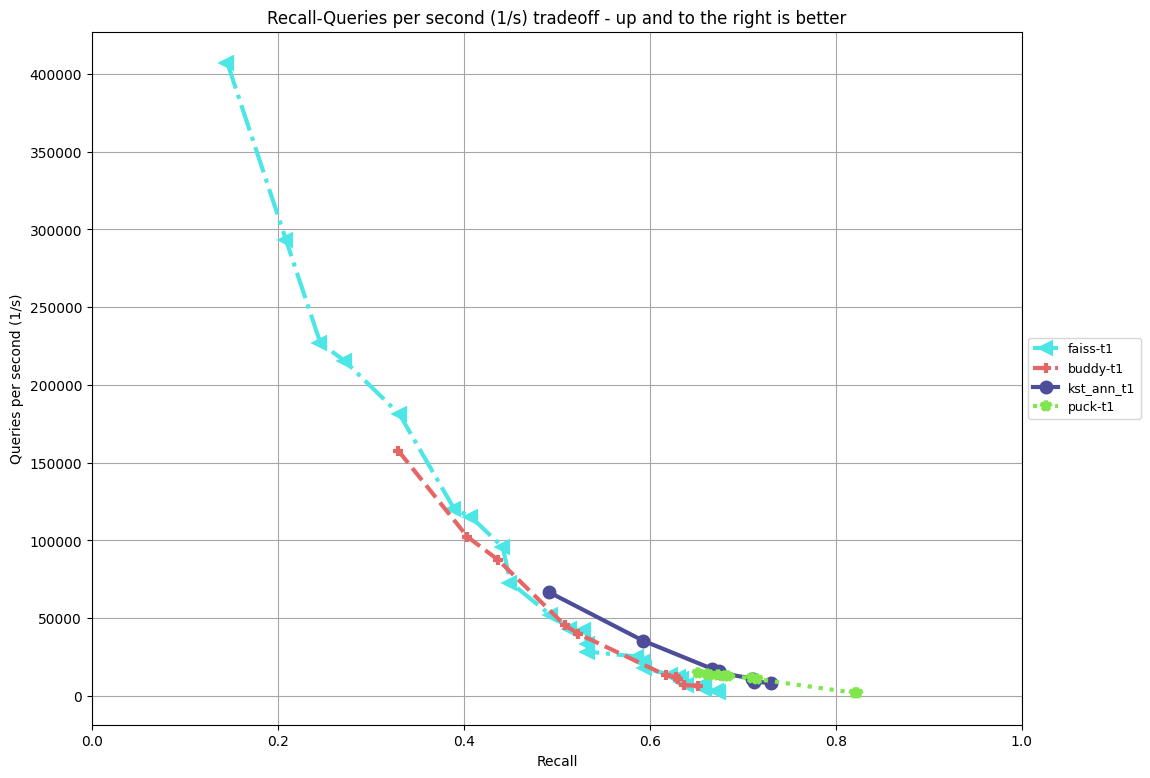
\includegraphics[width=\linewidth]{../t1_t2/results/T1/neurips21/bigann-1B.png}
      \caption{bigann-1B}
  \end{subfigure}
  \begin{subfigure}{10cm}
    \centering
    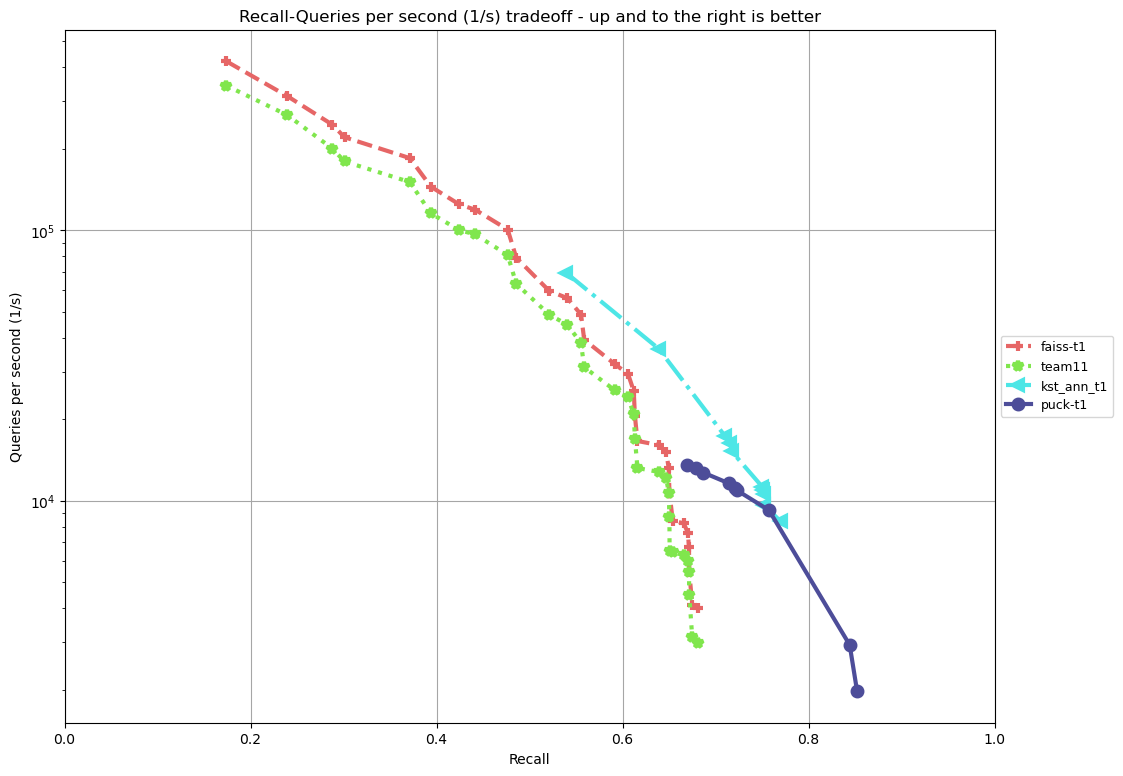
\includegraphics[width=\linewidth]{../t1_t2/results/T1/neurips21/deep-1B.png}
    \caption{deep-1B}
  \end{subfigure}
  \begin{subfigure}{10cm}
    \centering
    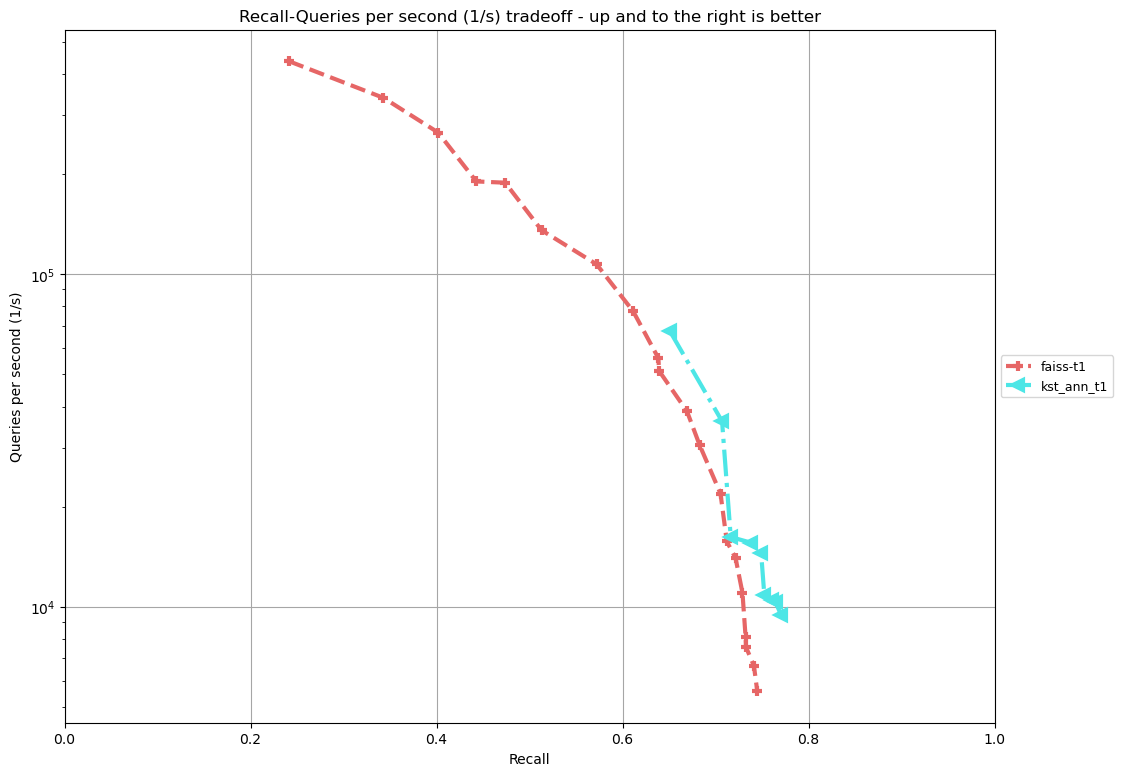
\includegraphics[width=\linewidth]{../t1_t2/results/T1/neurips21/msspacev-1B.png}
      \caption{msspacev-1B}
  \end{subfigure}
  \begin{subfigure}{10cm}
    \centering
    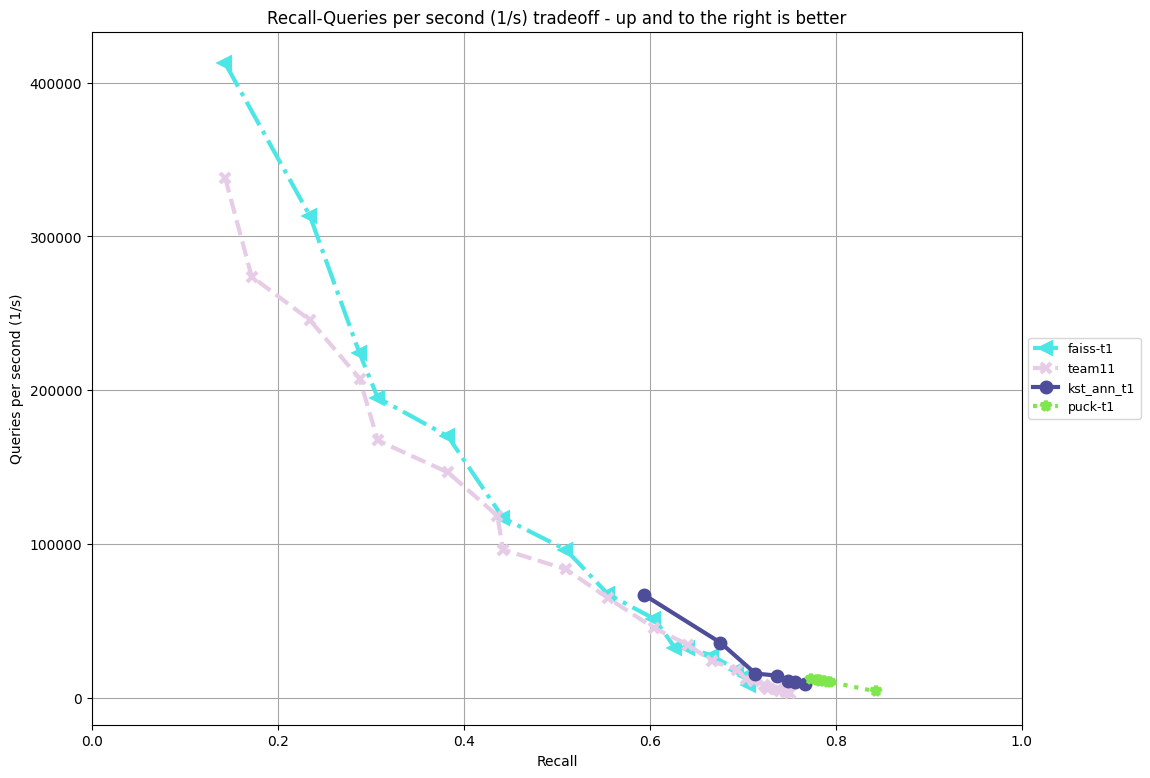
\includegraphics[width=\linewidth]{../t1_t2/results/T1/neurips21/msturing-1B.png}
    \caption{msturing-1B}
  \end{subfigure}
  \begin{subfigure}{10cm}
    \centering
    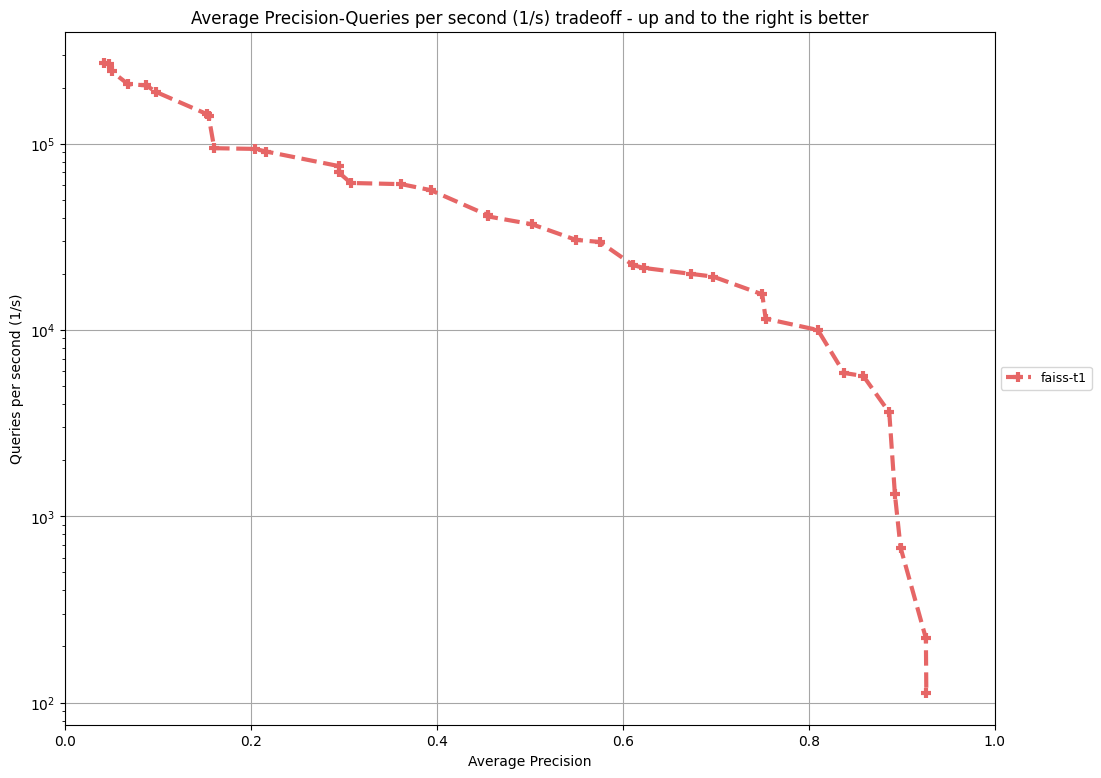
\includegraphics[width=\linewidth]{../t1_t2/results/T1/neurips21/ssnpp-1B.png}
      \caption{ssnpp-1B}
  \end{subfigure}
  \begin{subfigure}{10cm}
    \centering
    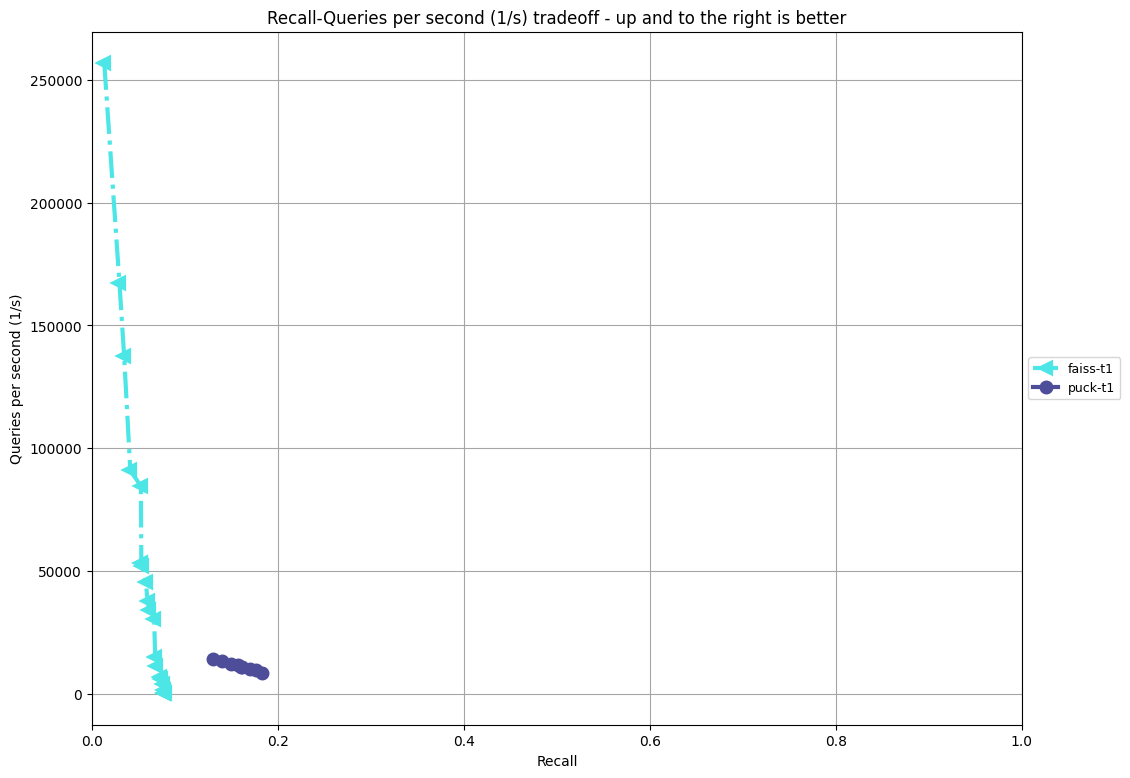
\includegraphics[width=\linewidth]{../t1_t2/results/T1/neurips21/text2image-1B.png}
    \caption{text2image-1B}
  \end{subfigure}
      
  \caption{QPS vs Recall plots for each dataset in Track T1.}
  
\end{figure}

\fi

\subsection{Track 2}
\begin{table}
  \caption{Leaderboard for Track T2. Recall achieved at 1500 QPS on Azure Ls8v2 VM with 8 vCPUs.}
  \begin{tabular}{l|c|c|c|c|c|c}
    \hline
    Algorithm & bigann-1B  & deep-1B & msspacev-1B & msturing-1B &   ssnpp-1B  &     text2image-1B \\
    \hline
    baseline &  0.94913 & 0.93706 & 0.90095 & 0.93564 & 0.16274 & 0.48854 \\
    \hline
    \href{https://github.com/harsha-simhadri/big-ann-benchmarks/pull/62}{kota-t2} & 0.950859 & & 0.904001 & 0.939817 & 0.18212 & \\
    \href{https://github.com/harsha-simhadri/big-ann-benchmarks/pull/6}{ngt-t2} & & & & & & \\
    \href{https://github.com/harsha-simhadri/big-ann-benchmarks/pull/70}{bbann} & & & 0.7602 & & 0.88573 & 0.495423 \\
    \hline
     
  \end{tabular}
  
\end{table}

\newcommand{\TtwoResPlot}[2]{
    \centering
    (#1) #2 \\
    \includegraphics[width=0.85\linewidth]{../t1_t2/results/T2/neurips21/#2.png} \\
}


\begin{figure}[ht]
\begin{minipage}{0.5\linewidth}
  \TtwoResPlot{a}{bigann-1B}
  \TtwoResPlot{b}{deep-1B}
  \TtwoResPlot{c}{msspacev-1B}
  \end{minipage}%
\begin{minipage}{0.5\linewidth} 
  \TtwoResPlot{d}{msturing-1B}
  \TtwoResPlot{e}{ssnpp-1B}
  \TtwoResPlot{f}{text2image-1B}
\end{minipage}
  \caption{QPS vs Recall plots for each dataset in Track T2::.}

\end{figure}

\iffalse 

\begin{figure}[ht]
  \begin{subfigure}{0.48\textwidth}
    \centering
    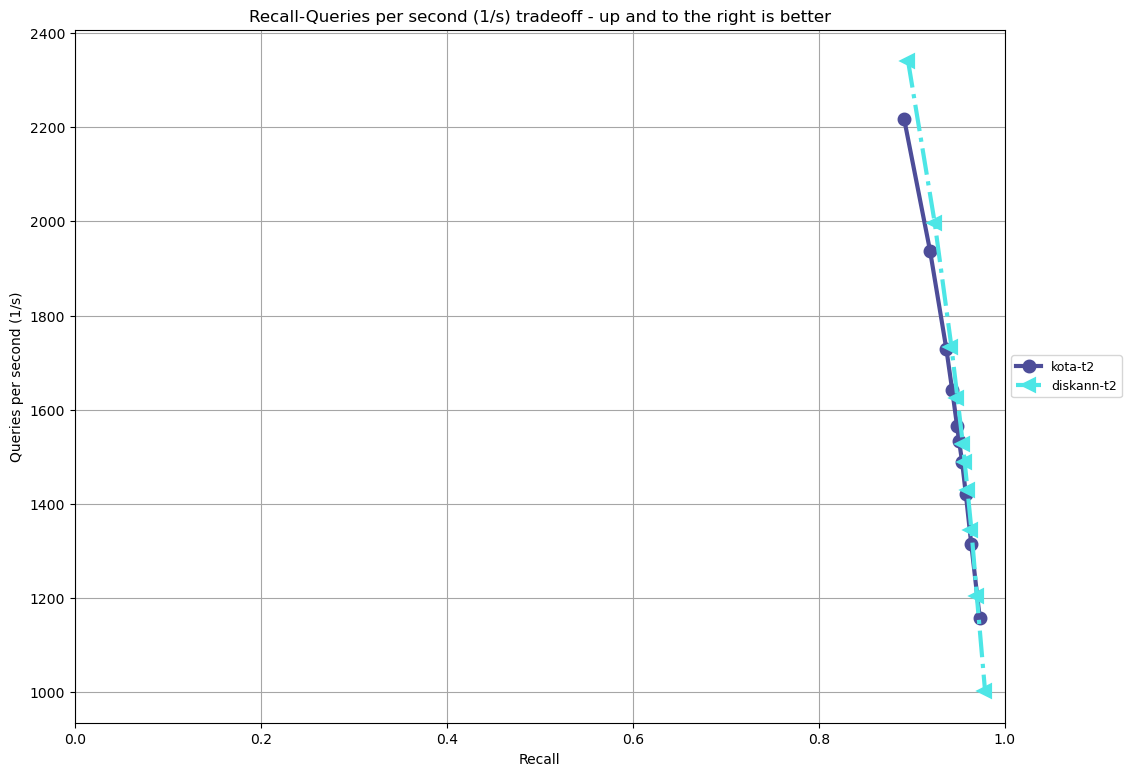
\includegraphics[width=\linewidth]{../t1_t2/results/T2/neurips21/bigann-1B.png}
      \caption{bigann-1B}
  \end{subfigure}
  \begin{subfigure}{0.48\textwidth}
    \centering
    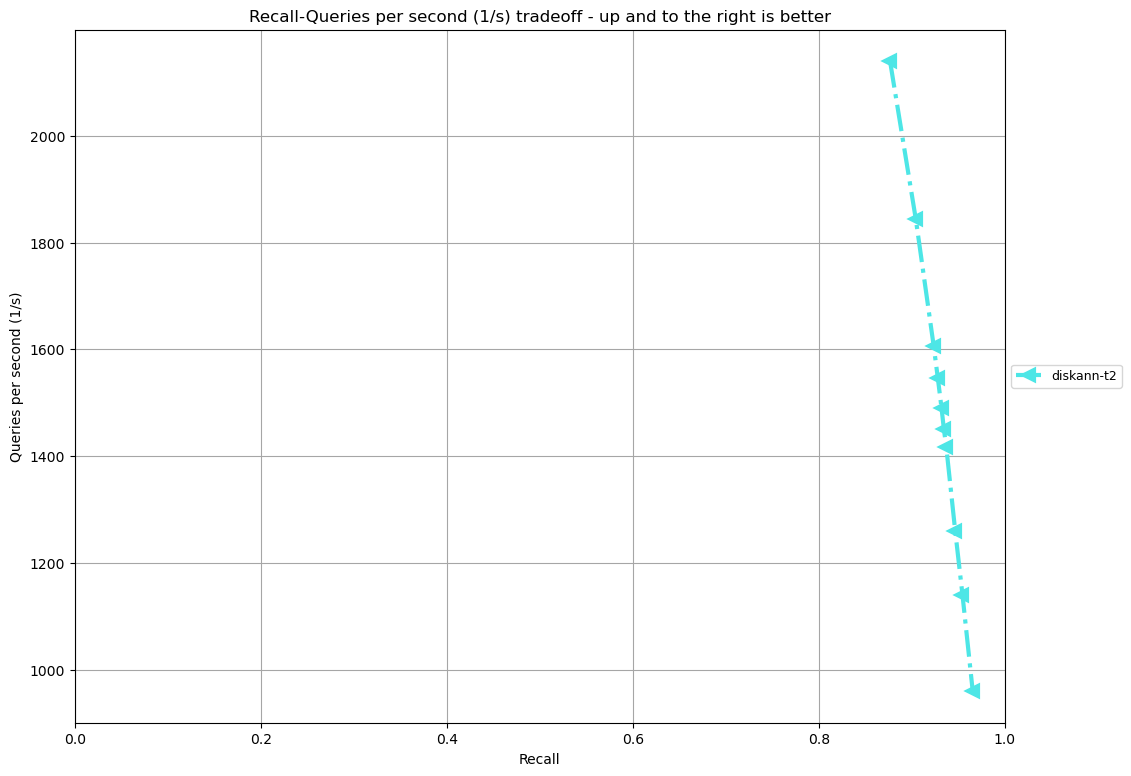
\includegraphics[width=\linewidth]{../t1_t2/results/T2/neurips21/deep-1B.png}
    \caption{deep-1B}
  \end{subfigure}
  \begin{subfigure}{0.48\textwidth}
    \centering
    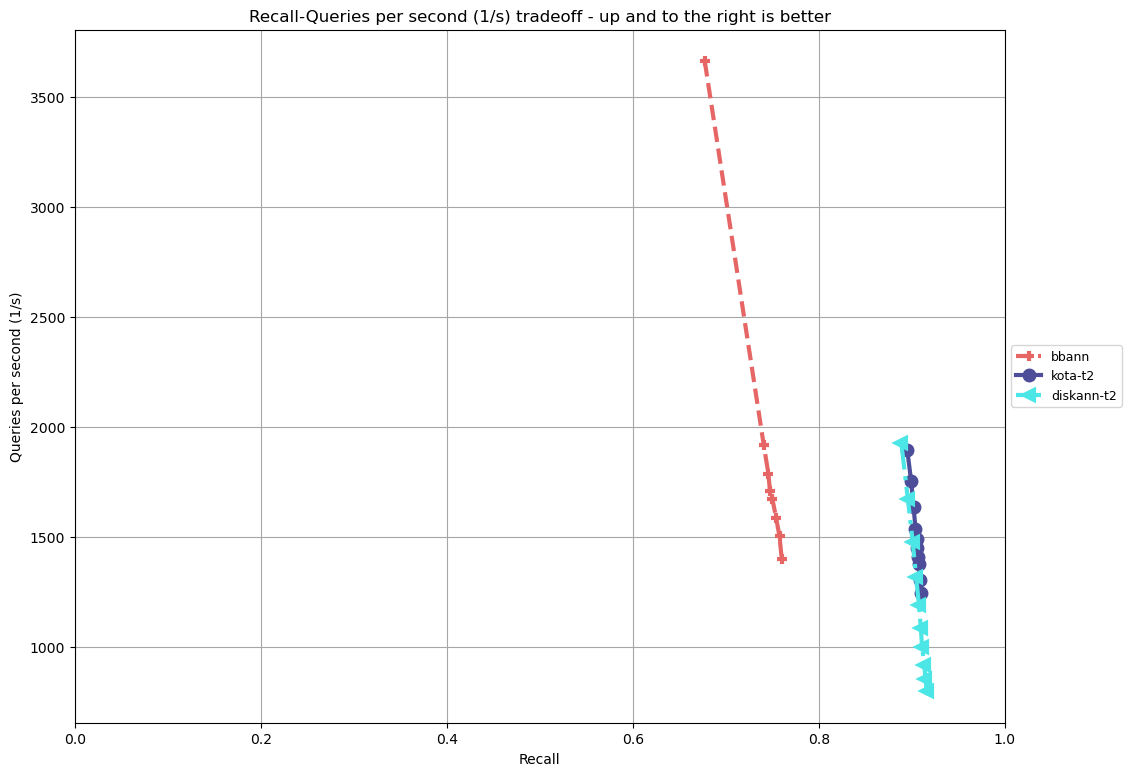
\includegraphics[width=\linewidth]{../t1_t2/results/T2/neurips21/msspacev-1B.png}
      \caption{msspacev-1B}
  \end{subfigure}
  \begin{subfigure}{0.48\textwidth}
    \centering
    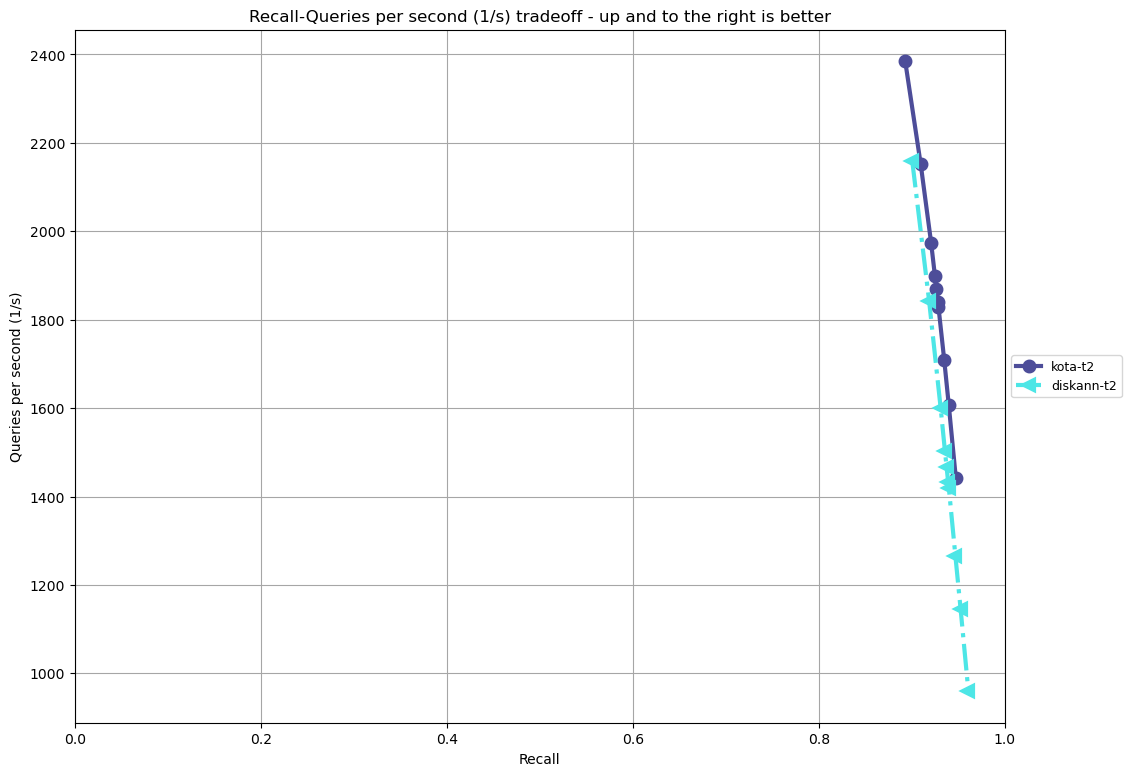
\includegraphics[width=\linewidth]{../t1_t2/results/T2/neurips21/msturing-1B.png}
    \caption{msturing-1B}
  \end{subfigure}
  \begin{subfigure}{0.48\textwidth}
    \centering
    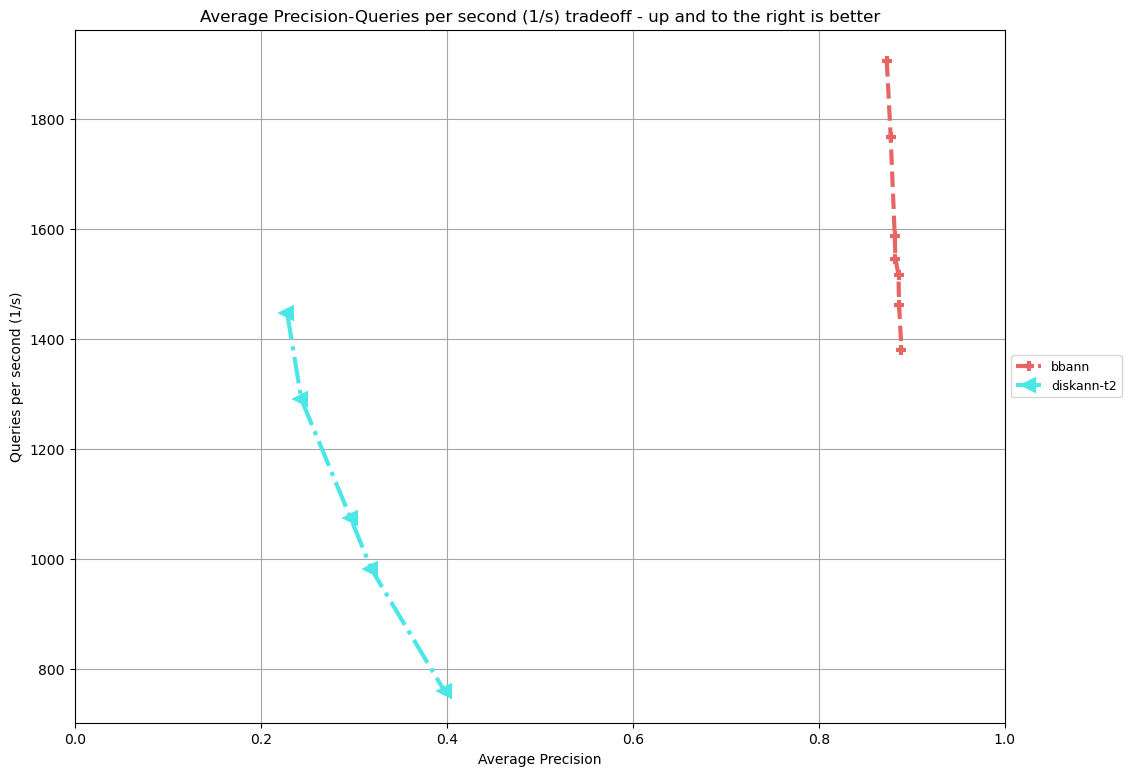
\includegraphics[width=\linewidth]{../t1_t2/results/T2/neurips21/ssnpp-1B.png}
      \caption{ssnpp-1B}
  \end{subfigure}
  \begin{subfigure}{0.48\textwidth}
    \centering
    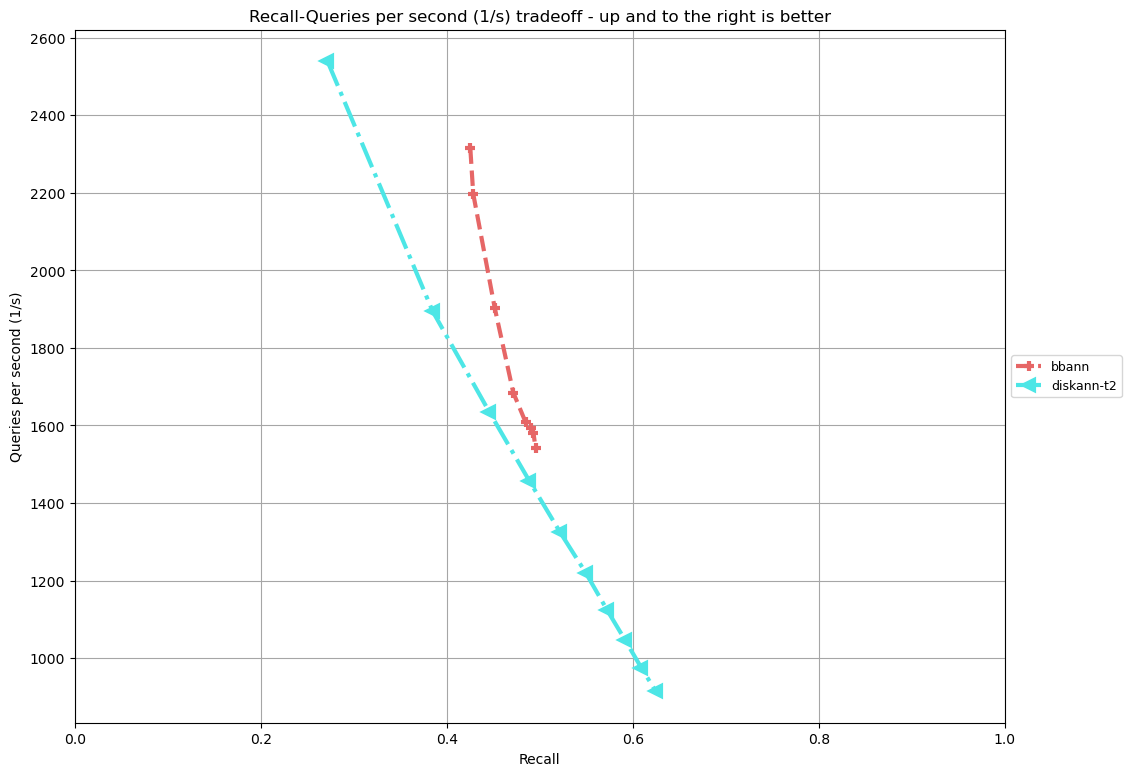
\includegraphics[width=\linewidth]{../t1_t2/results/T2/neurips21/text2image-1B.png}
    \caption{text2image-1B}
  \end{subfigure}
      
  \caption{QPS vs Recall plots for each dataset in Track T2::.}

\end{figure}

\fi 

\subsection{Track 3}




\bibliographystyle{plain}
\bibliography{ref}


\end{document}
